\section{Evaluation}

\begin{figure*}[tbp]
     \centering
     \begin{subfigure}[b]{0.33\textwidth}
        \centering
        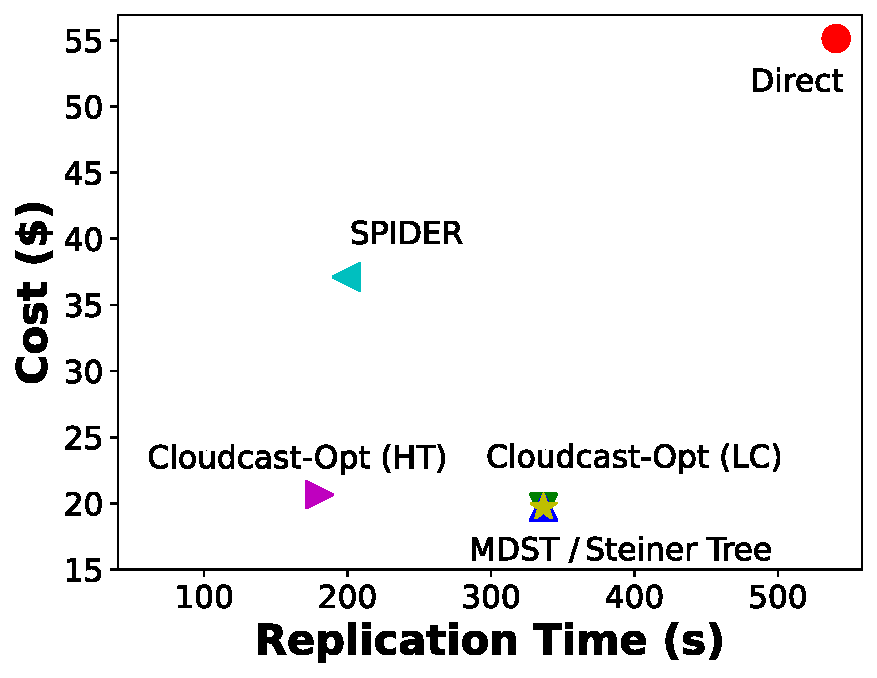
\includegraphics[width=\textwidth]{figures/aws.pdf}
        \caption{AWS Intra-Cloud}
        \label{fig:aws-intra-cloud}
    \end{subfigure}
    \hfill
    \begin{subfigure}[b]{0.33\textwidth}
        \centering
        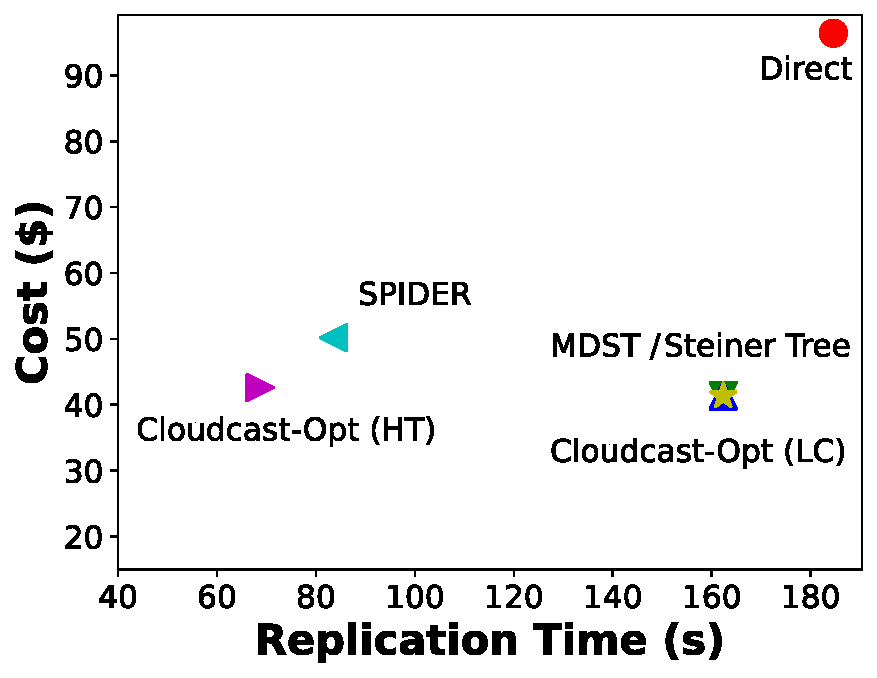
\includegraphics[width=\textwidth]{figures/azure.pdf}
        \caption{Azure Intra-Cloud}
        \label{fig:azure-intra-cloud}
    \end{subfigure}
    \hfill
    \begin{subfigure}[b]{0.33\textwidth}
        \centering
        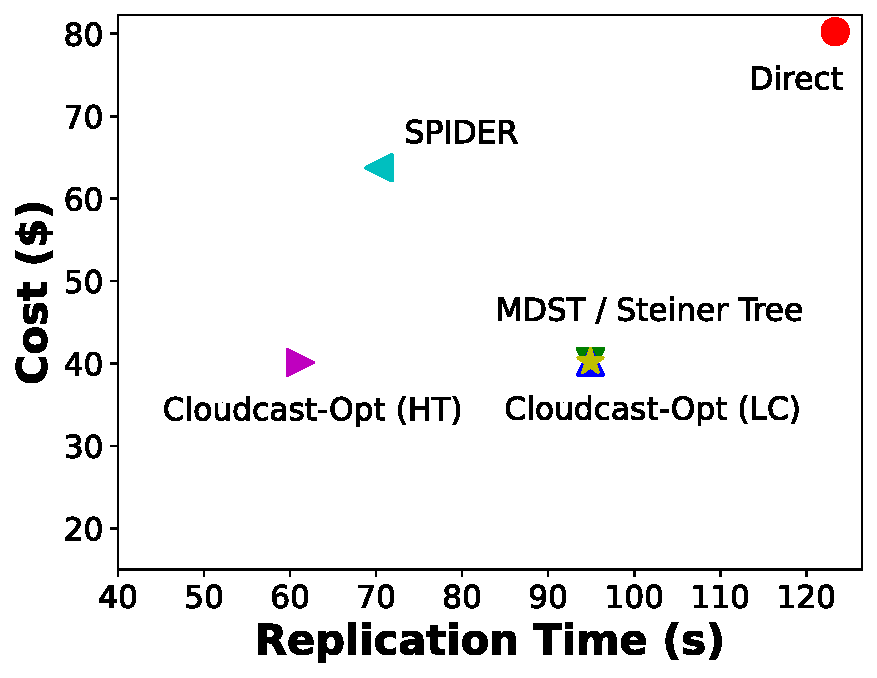
\includegraphics[width=\textwidth]{figures/gcp.pdf}
        \caption{GCP Intra-Cloud}
        \label{fig:gcp-intra-cloud}
    \end{subfigure}
    \hfill
    %\vspace{-2em}
    \caption{Intra-cloud multicast results for algorithms implemented on \sys{}.  
    %In all cases \sys{}-Opt is able to find significantly faster low-cost solutions where compared with existing techniques.  Furthermore, the MDST/Steiner Tree solution using ephemeral waypoints is able to consistently find the cost-optimal solution.  
    % \shu{we need to explain why we use these topologies, as well as why there are some variances in the running outcomes (e.g. SPIDER is closer to Cloudcast in Azure, or AWS runtime is much worse than the other cloud)}
    }
    \label{fig:intra-cloud}
\end{figure*}
\begin{figure}[tbp]
    \centering
    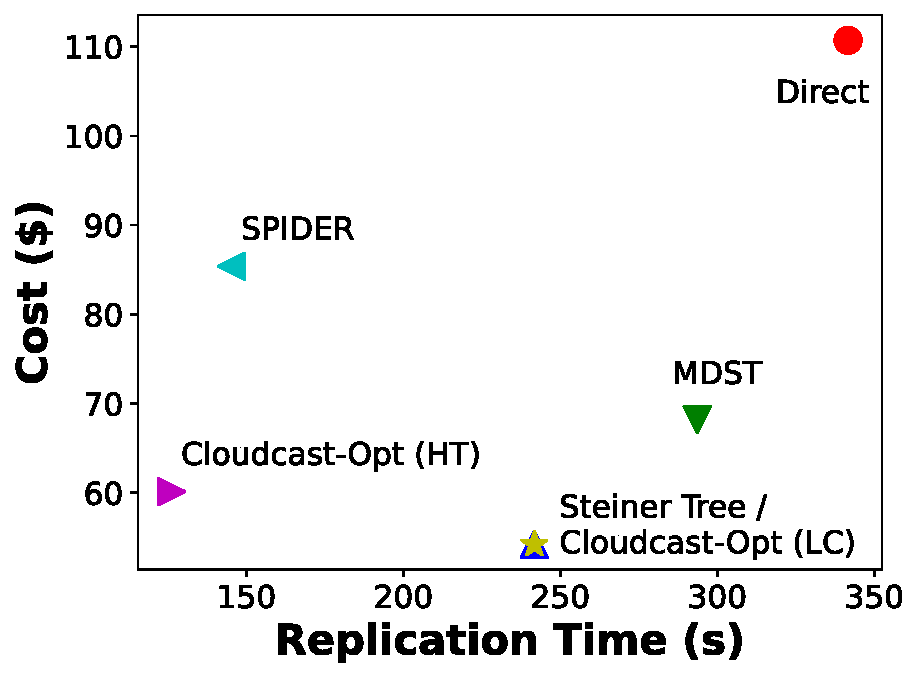
\includegraphics[width=
    0.33\textwidth]{figures/inter_cloud.pdf}
    \caption{Inter-cloud multicast results for different algorithms implemented on \sys{}. The \sys{} replication tree is visualized in Figure \ref{fig:example-topo}.
    % \joey{Figures should have a clear "takeaway" in the caption.  What would you say if presenting this figure in a talk.}
    }
    \label{fig:inter-cloud-1}
\end{figure}

In this section, we evaluate \sys{} across three metrics: replication cost, replication time, and the optimizer solve time (or simply, runtime).
% 
In particular, we show that for intra-cloud and inter-cloud bulk data transfer, \sys{} is able to achieve up to 61.5\% cost improvements under a tight runtime budget when compared to academic, commercial, and open-source baselines.
% 
We also show that our approximations to reduce the optimizer solve time (as discussed in \cref{ss:approximations}) are highly effective by reducing the runtime by on average 30.68$\times$ for 5-destination replications.

% In the rest of this section, we focus on answering the following questions: 
% \begin{enumerate} 
%     \item How do the multicast trees computed by our optimizer compare to previous algorithmic solutions for multicast in terms of total cost and replication time?
%     % for intra- and inter-cloud transfers? 
%     (Section \ref{sec:algorithm_eval})
%     \item How does \sys{} perform compared to existing commercial (e.g. AWS multi-bucket replication) and open-source systems (e.g. BitTorrent) in terms of total cost and replication time? (Section \ref{sec:sys_eval})
%     \item How do our approximation methods affect our optimizer solve time and solution quality? (Section \ref{sec:solution_qual_eval})
% \end{enumerate}
% \begin{subfigure}[b]{0.45\textwidth}
    %     \centering
    %     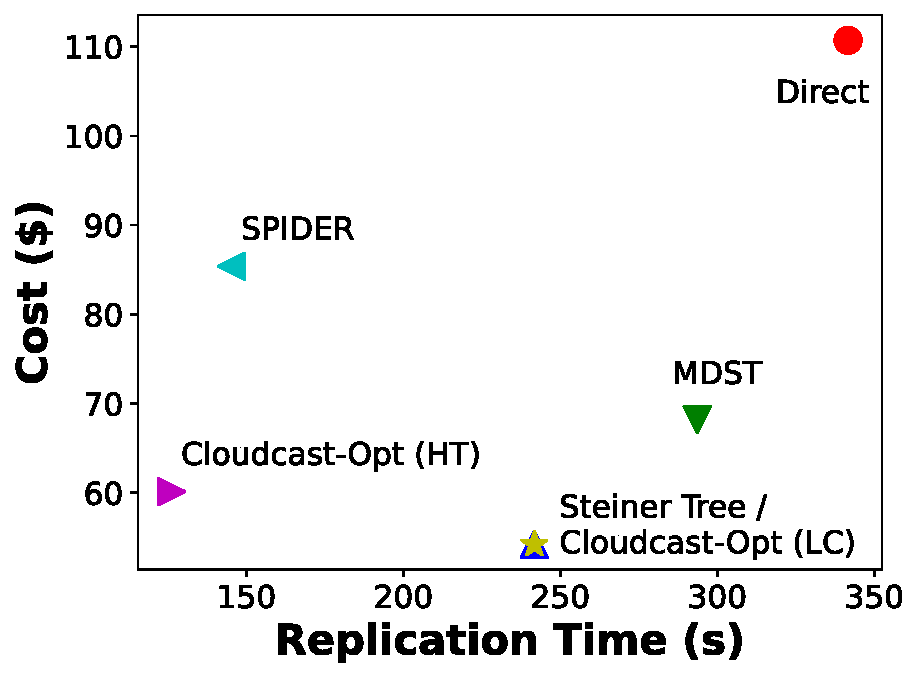
\includegraphics[width=\textwidth]{figures/inter_cloud.pdf}
    %     \caption{\textbf{Multi-cloud}}
    %     \label{fig:inter-cloud-1}
    % \end{subfigure}

\subsection{Comparing Planner Algorithms} \label{sec:algorithm_eval}

In this section, we evaluate different algorithms for determining multicast trees for data replication. We implement each of the following algorithms inside \sys{}'s planner, and compare the end-to-end replication time and cost for both intra-cloud and inter-cloud transfers using AWS, GCP, and Azure cloud services:  
\begin{itemize}
    \item \textbf{Direct}: Data is transferred directly from the source to the destination regions.  
    \item \textbf{MDST}: Data is transferred along edges selected by a Minimum Directed Spanning Tree (including source and destination regions) computed from network costs. 
    \item \textbf{Stiener Tree}: Data is transferred along edges selected by a Steiner tree (including optional waypoint regions) computed from network costs. 
    % \item \textbf{Bullet}\cite{kostic2003bullet}: Data is transferred according to the plan generated by Bullet, a high bandwidth data dissemination technique using an overlay mesh. 
    \item \textbf{SPIDER} \cite{ganguly2005fast}: Data is transferred according to the plan generated by SPIDER, an academic baseline designed for fast bulk replication to multiple destinations.
    \item \textbf{Cloudcast-Opt}: Data is transferred along the cost-optimized multicast tree generated by our optimizer given a replication time constraint. \shu{I remove the low-cost optimizer here if we are not including it into in-network eval}
    % \item \textbf{Optimizer (Low-cost)}: Cost-optimized topology generated from a high replication time constraint. 
\end{itemize}
% \sys{} has a centralized control plane for determining overlay nodes and distribution trees prior to initiating replication. To compare to peer-to-peer systems such as Bullet, which often dynamically determine distribution trees, we simulate what the distribution trees a P2P system would have generated to centrally determine the corresponding configuration for \sys{}.

For the baseline algorithms, there is no mechanism for selecting how many VMs to create in each region. Thus, we create the maximum number of VMs available in regions through which the data traverses. For example, if a waypoint region is selected by the Steiner tree, we create the maximum possible number of VMs in that region as our overlay routers. \shu{is it true, or do we want to say something like fixed # of vms} 

\subsubsection{Cloud Experiments}
\label{ss:cloud-exp}
On top of \sys{}, we compare the replication time and cost of different multicast algorithms for replicating 100GB data from 1 source to 6 destination regions. Due to the high cost of running data multicast in the cloud, we select a single representative example that contains source regions with high egress costs to demonstrate the potential cost savings. We choose the following configurations to evaluate:  \textbf{AWS Intra-Cloud} (from \path{ap-east-1} to \path{us-west-1}, \path{ap-northeast-3}, \path{eu-north-1}, \path{ap-south-1}, \path{ca-central-1}, \path{ap-northeast-1}), \textbf{Azure Intra-Cloud} (from \path{brazilsouth} to \path{westeurope}, \path{westus}, \path{koreacentral}, \path{australiaeast}, \path{uaenorth}, \path{centralindia}), \textbf{GCP Intra-Cloud} (from \path{asia-southeast2-a} to \path{australia-southeast1-a}, \path{southamerica-east1-a}, \path{europe-west4-a}, \path{europe-west6-a}, \path{asia-east1-a}, \path{europe-west2-a}), and \textbf{Inter-Cloud} (from \path{gcp:asia-southeast1-a} to \path{azure:australiaeast}, \path{azure:eastasia}, \path{aws:ap-southeast-2}, \path{azure:brazilsouth}, \path{aws:sa-east-1}, \path{gcp:australia-southeast1-a}).

% The setups for evaluation are as follows:  
% \begin{itemize}
%     \item \textbf{AWS Intra-Cloud:} From \path{ap-east-1} to \path{us-west-1}, \path{ap-northeast-3}, \path{eu-north-1}, \path{ap-south-1}, \path{ca-central-1}, \path{ap-northeast-1} all in AWS.
%     \item \textbf{Azure Intra-Cloud:} From \path{brazilsouth} to \path{westeurope}, \path{westus}, \path{koreacentral}, \path{australiaeast}, \path{uaenorth}, \path{centralindia} all in Azure.
%     \item \textbf{GCP Intra-Cloud:} From \path{asia-southeast2-a} to \path{australia-southeast1-a}, \path{southamerica-east1-a}, \path{europe-west4-a}, \path{europe-west6-a}, \path{asia-east1-a}, \path{europe-west2-a} all in GCP
%     \item \textbf{Inter-Cloud:}  From \path{gcp:asia-southeast1-a} to \path{azure:australiaeast}, \path{azure:eastasia}, \path{aws:ap-southeast-2}, \path{azure:brazilsouth}, \path{aws:sa-east-1}, \path{gcp:australia-southeast1-a}
% \end{itemize}

% To demonstrate the potential cost-saving, we select source regions with particularly high egress costs. 

% We discuss the generalizability of our approach via simulations in Section \ref{sec:simulated_section}.  

% We show and discuss aggregated results overly randomly selected source and destination regions in \cref{random-ablation}.  

% \sarah{Find best case comparison for SPIDER, MDST, and NDirect}

% We show our intra-cloud results for AWS, GCP, and Azure in Figure \ref{fig:aws-intra-cloud}, \ref{fig:azure-intra-cloud}, \ref{fig:gcp-intra-cloud} respectively. These figures show that \sys{}-Opt can achieve $50-62.4\%$ cost reductions and $2-2.84\times$ replication time speedup compared to naive data transfer to all destinations via direct paths. SPIDER is an algorithm designed for high-bandwidth data distribution; it is shown to have the lowest replication time among all the baselines. However, as SPIDER is not cost-aware, \sys{}-Opt solution can achieve $28.4-44.0\%$ cost savings while still having $1.11-1.35\times$ replication speedup compared to this algorithm. 

We show our intra-cloud replication results for AWS, GCP, and Azure in Figure \ref{fig:aws-intra-cloud}, \ref{fig:azure-intra-cloud}, \ref{fig:gcp-intra-cloud} respectively, and inter-cloud results in Figure \ref{fig:inter-cloud-1}. For both intra-cloud and inter-cloud experiments, \sys{}-Opt solution leads to $46-62.4\%$ cost reductions and $2-2.84\times$ replication time speedup compared to naive data transfer to all destinations via direct paths. SPIDER is an algorithm designed for high-bandwidth data distribution, and it is shown to have the lowest replication time among all baselines in our experiment setups. However, as SPIDER is not cost-aware, \sys{}-Opt can achieve $28.4-44.0\%$ cost savings while still maintaining $1.11-1.35\times$ replication speedup compared to this algorithm. 

We run \sys{}-Opt with only a single replication time budget, but we note that \sys{}-Opt is able to find multiple points on the cost-replication time Pareto frontier. In fact, \sys{}-Opt can generate an equivalent cost-minimizing multicast plan as the Steiner Tree, given a loose replication time budget. What distinguishes \sys{}-Opt from the Steiner Tree is the ability to trade off cost and replication and to also select the lowest replication time solution among cost-equivalent Steiner Trees. For example, for GCP and Azure intra-cloud transfer, \sys{}-Opt is able to identify a multicast replication tree of the same cost with $2.5\times$ and $1.6\times$ replication speedup compared to the Steiner Tree. 

% SPIDER’s algorithm achieves the best through- put amoung baselines, but Cloudcast still achieves 29.6\% cost savings compared to SPIDER, and 1.15× speedup com- pared to SPIDER, and 45.7\% cost savings and 2.71× speedup compared to the direct baseline. 

% \sarah{we can't call steiner tree a baseline does it work? yeah I would try to tighten this sectup becaise we re short on spac e, and the diagrams kinda get the point across} okay will remove some text here

%On the other hand, Steiner Tree is an algorithm that is cost-optimal but bandwidth-agnostic. Evaluations have shown that \sys{}-Opt is able to identify a cost-optimal multicast tree for tighter runtime budgets. For example, for GCP and Azure intra-cloud transfer, Cloudcast identifies a same-cost replication solution with 2.5$\times$ and 1.6$\times$ replication speedup, respectively, when compared to Steiner Tree. For intra-cloud experiments, waypoint regions are less likely to improve cost (we note this is not always the case for intra-cloud replication), so the MDST and Steiner Tree solutions are also equivalent. However, for the inter-cloud replication, the use of waypoint regions by the Steiner Tree (and also \sys{}-Opt’s low-cost solution) results in a 20.5\% cost saving and 1.2$\times$ speedup compared to MDST. 

% \shu{I think here the comparisons might be incomplete}

% To summarize: compared to the baseline algorithms described above, our solution can achieve $1.1$-$2.84$$\times$ replication time speedup with $28.4$-$62.4$\% cost reductions for 100GB intra- and inter-cloud data transfer\sarah{I think this is redundant }


\subsubsection{Simulated Experiments}
To understand how our optimizer behaves for different selections of source and destination regions and different target replication times, we run simulated ablations. \label{sec:simulated_section}

\heading{Varying Target Replication Time}
To understand how \sys{}'s optimizer compares to other algorithms under varying target replication time inputs, we run an ablation where we vary the target replication time to identify the Pareto curve identified by our optimizer. We show this curve in Figure \ref{fig:pareto}, which shows our optimizer outperforms baseline algorithms for all replication time inputs. A high replication budget eventually converges to the Steiner Tree solution (which is sometimes equivalent to the MDST solution, depending on the set of source and destination nodes).  

\begin{figure}[t]
    \centering
    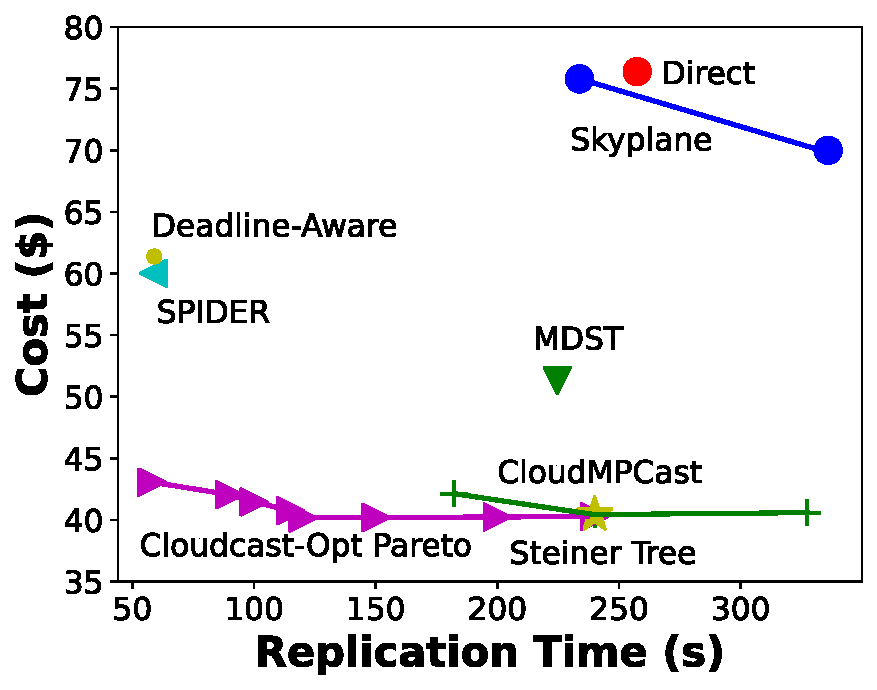
\includegraphics[width=.75\linewidth]{figures/pareto.pdf}
    \caption{\textbf{Simulated results for Cloudcast-Opt Pareto curve comparing to baselines. \shu{considered adding a point for Nxskyplane here}}}
    \label{fig:pareto}
\end{figure}


\heading{Varying Region Selection}
\label{random-ablation}
We test the generality of our improvements by randomly selecting source and destination regions for varying numbers of destinations. We show aggregated results over 100 samples for different numbers of destinations in Figure \ref{fig:dest_ablation}. \sys{} is able to improve the runtime and cost of replication consistently across varying numbers of destinations. The average improvement (as well as the variation in the improvement) increases with more destinations, as this increases the search space for the optimizer to discover faster, cheaper replication trees. 

% \begin{figure}[t]
%     \centering
%     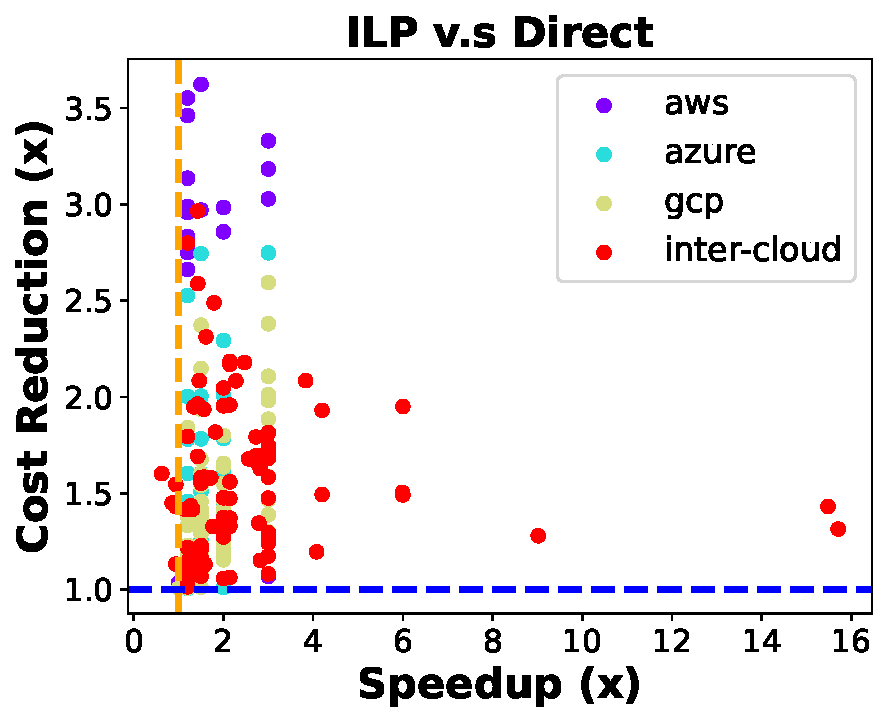
\includegraphics[width=.75\linewidth]{figures/6_dest_100_config.pdf}
%     \caption{\textbf{Simulation: 6 destinations, randomly sampled 100 configurations for Intra-aws/azure/gcp and Inter-cloud transfer)}}
%     \label{fig:random-6-dest}
% \end{figure}


% \begin{figure}[t]
%     \centering
%     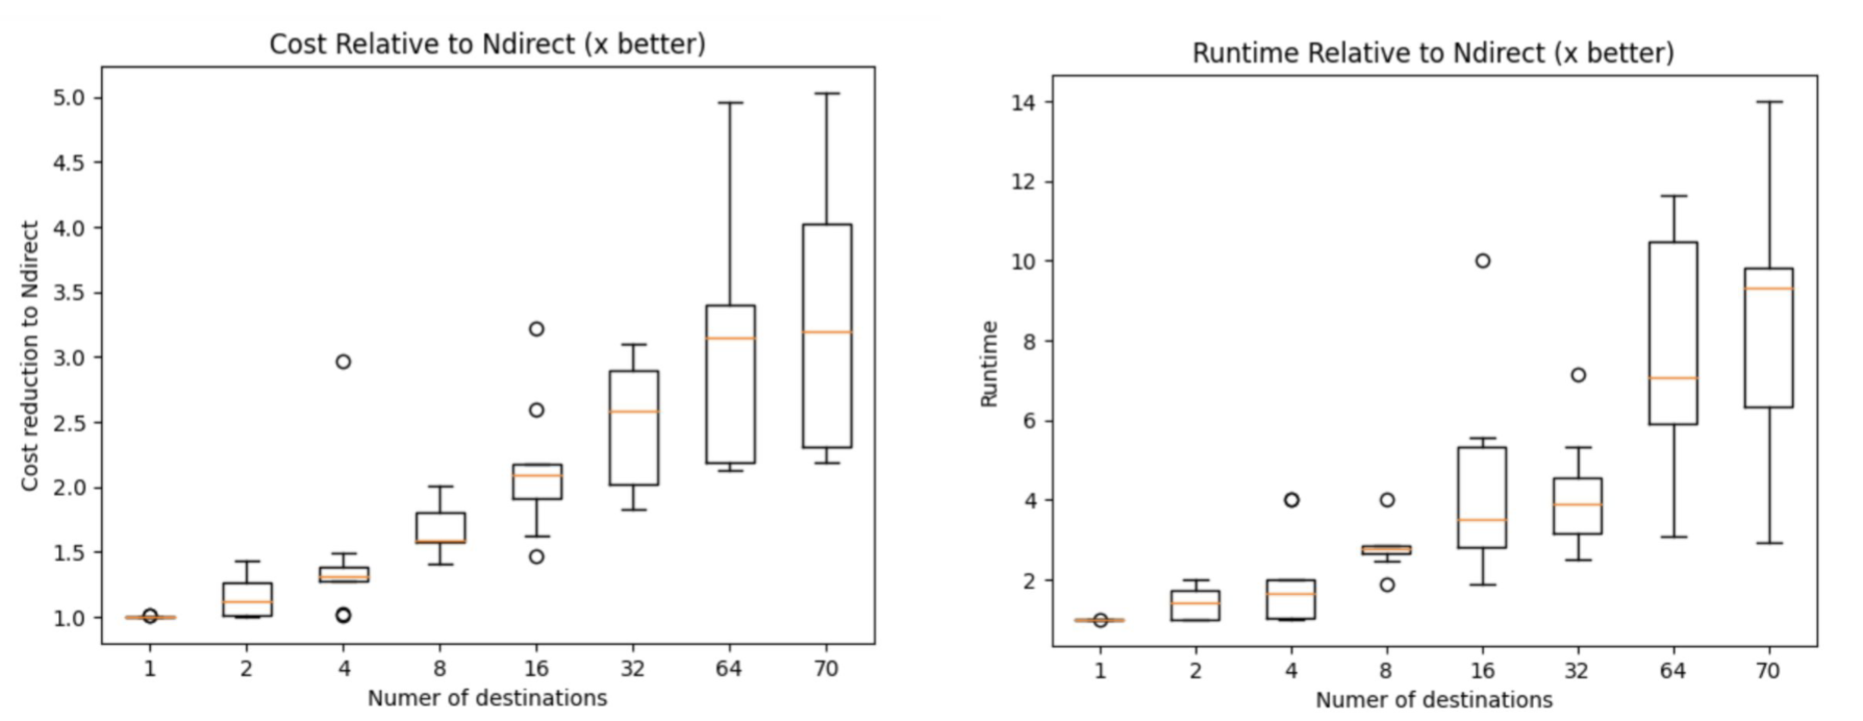
\includegraphics[width=.5\linewidth]{figures/dest_ablation.pdf}
%     \caption{\sys{} optimizer's cost and runtime improvement over direct replication for randomly sampled source and destination regions for varying numbers of destinations.} \label{fig:dest_ablation}
%     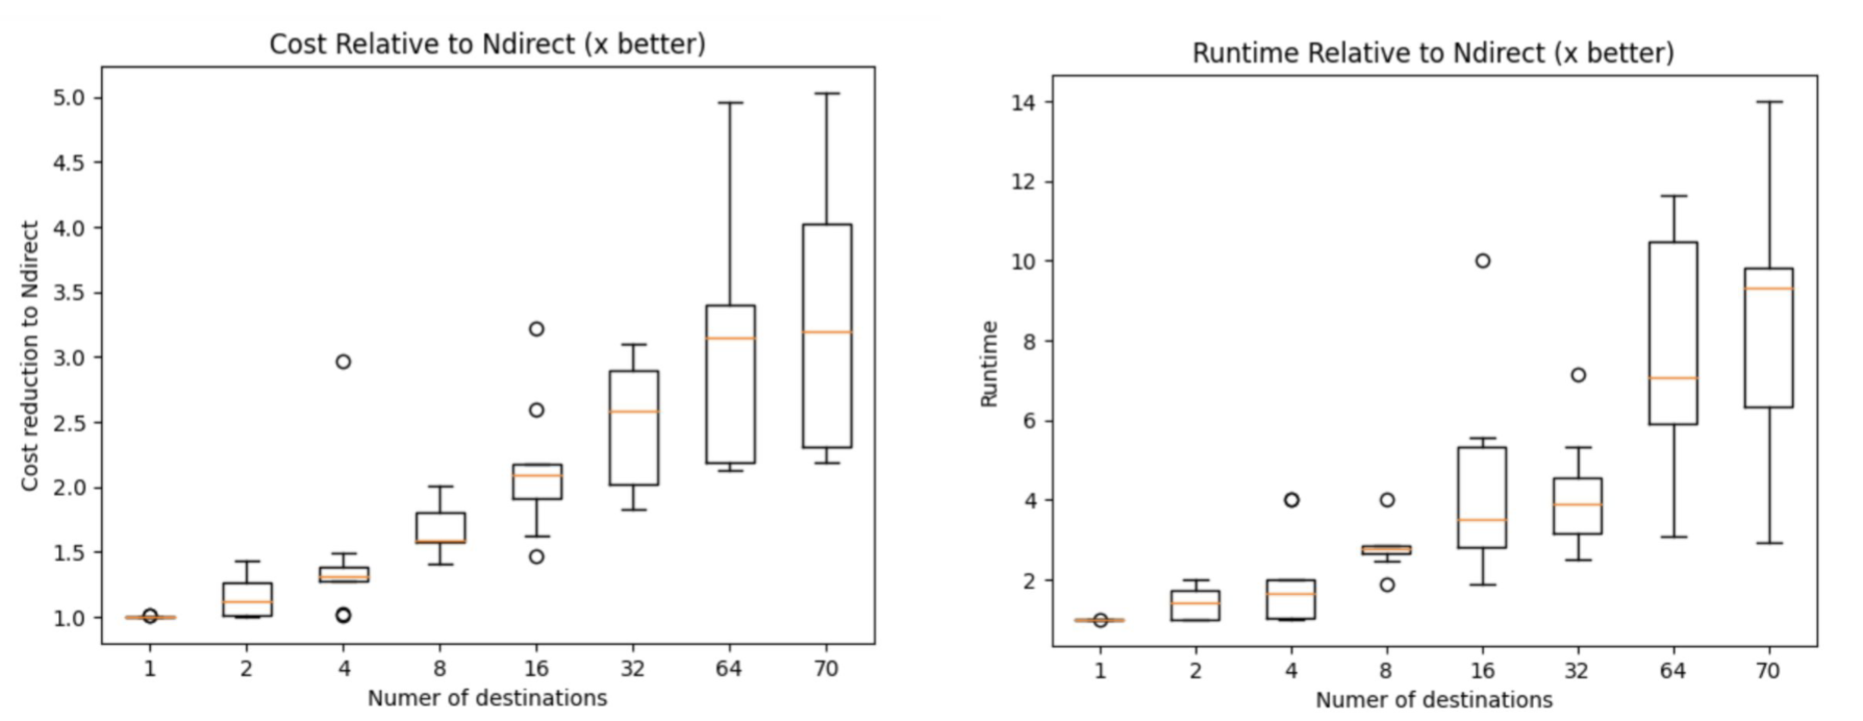
\includegraphics[width=.5\linewidth]{figures/dest_ablation.pdf}
% \end{figure}


\begin{figure}[t]
\centering
\subfloat[][Cost Reduction]{
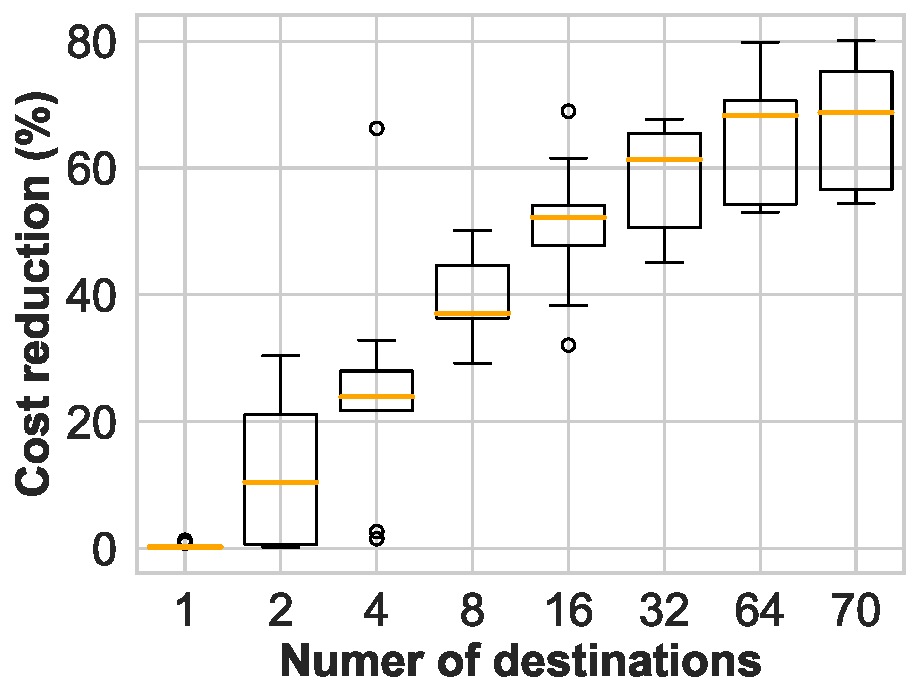
\includegraphics[width=.5\linewidth]{figures/ilp_vary_dest_ndirect_cost_reduction.pdf}\label{fig:dest_ablation1}
} 
\subfloat[][Replication Time Speedup]{
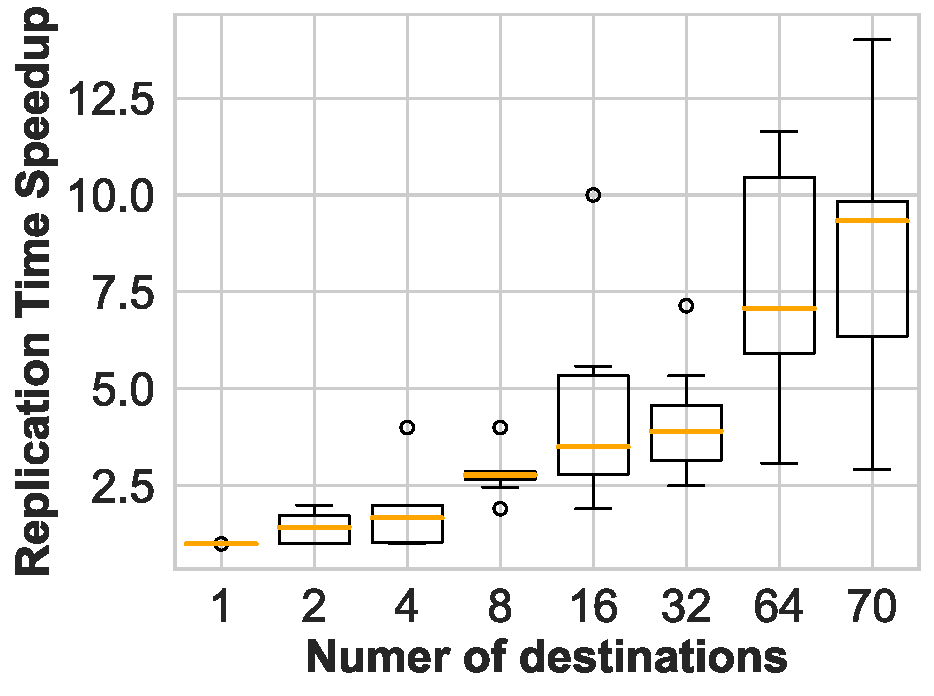
\includegraphics[width=.5\linewidth]{figures/ilp_vary_dest_ndirect_runtime_speedup.pdf}\label{fig:dest_ablation2}
}
\caption{\sys{} optimizer's cost and replication time improvement over direct replication for randomly sampled source and destination regions for varying numbers of destinations.} \label{fig:dest_ablation}
\end{figure}



\subsection{Cloudcast v.s. Other Systems} \label{sec:sys_eval}
We run end-to-end evaluation comparing \sys{} with a commercial baseline (AWS multi-region bucket replication) and P2P systems (Bittorrent and Bullet). 

\subsubsection{Commercial baseline: S3 Multi-Region bucket replication}
% We run an end-to-end comparison between \sys{} and AWS's multi-region bucket replication for single-provider multicast. AWS support adding multiple replication rules to a source bucket to specify automatic replication to one or more replication buckets. AWS supports a replication time control with a minimum 15-minute SLO, however, we found in our experiments that replicated is typically completed much faster, and use the actual replication time as a point of comparison. 

% To evaluate AWS replication time, we create buckets with replication rules from source to destination buckets. Once the replication rules are created, we copy data from a bucket in the same region into the source bucket with 16 VMs. After the write completes, we measure the time until replication into all destination buckets. We calculate the transfer cost according to AWS's pricing page, \textcolor{red}{(TODO: cite)}. 

% We compare AWS's replication time and cost to \sys{} using three topology algorithms: a direct topology (each destination receives data from the source), an optimizer topology configured with high throughput, and an ILP topology configured with low throughput. We transfer a 66 billion parameter OPT model \cite{zhang2022opt} ($122$GB across 9 files) from \texttt{aws:ap-east-1} to \texttt{aws:ap-southeast-2}, \texttt{aws:ap-south-1}, \texttt{aws:ap-northeast-3}, \texttt{aws:ap-northeast-2}, \texttt{aws:ap-northeast-1}. We configure the optimizer to meet a job completion time similar to AWS's replication time, showing about 3X cost reduction in \ref{fig:aws_comparison}. 
We run an end-to-end comparison between \sys{} and AWS's multi-region bucket replication\cite{aws-replication} for single-provider multicast.
AWS supports adding multiple replication rules to a source bucket to specify automatic replication to one or more replication buckets. 
% NOTE: below line added by Simon
In comparison, GCP and Azure only support point-to-point transfers and do not provide a data replication product that supports multiple destinations. GCP's multi-region bucket does not explicitly transfer to multiple destinations and it is bounded by geographical regions. \todo{cite gcp/azure pages}
In the aspect of time control, AWS supports a replication time control with a minimum 15-minute SLO. However, we found that in our experiments replications typically completed much faster than 15 minutes. Therefore, we use the actual replication time as a point of comparison. 



We compare AWS's replication time and cost to \sys{} with the planner implemented with both direct transfer and the optimizer. 
We transfer an OPT model\cite{zhang2022opt} with 66 billion parameters ($122$GB in total across 9 files) from \path{aws:ap-east-1} to \path{aws:ap-southeast-2}, \path{aws:ap-south-1}, \path{aws:ap-northeast-3}, \path{aws:ap-northeast-2}, \path{aws:ap-northeast-1}. To evaluate AWS replication time and cost, we create buckets with replication rules from a bucket in the source region to buckets in destination regions. 
Once the replication rules are created, we copy data from a bucket in the same region into the source bucket with 16 VMs. After the write completes, we measure the time until the completion of replication into all destination buckets. We calculate the transfer cost according to AWS's pricing page \cite{aws-data-transfer-cost}. We compare AWS multibucket replication to \sys{} implemented with both the direct and optimizer planner and running.  As shown in Figure \ref{fig:aws_comparison}, the direct transfer has the same egress costs as AWS bucket replication, but the VM costs are much less than the service fee charged by AWS for the replication. Overall, \sys{} with the optimizer is able to achieve $2.3\times$ replication speedup and $61.5\%$ cost savings. 

\begin{figure}[t]
    \centering
    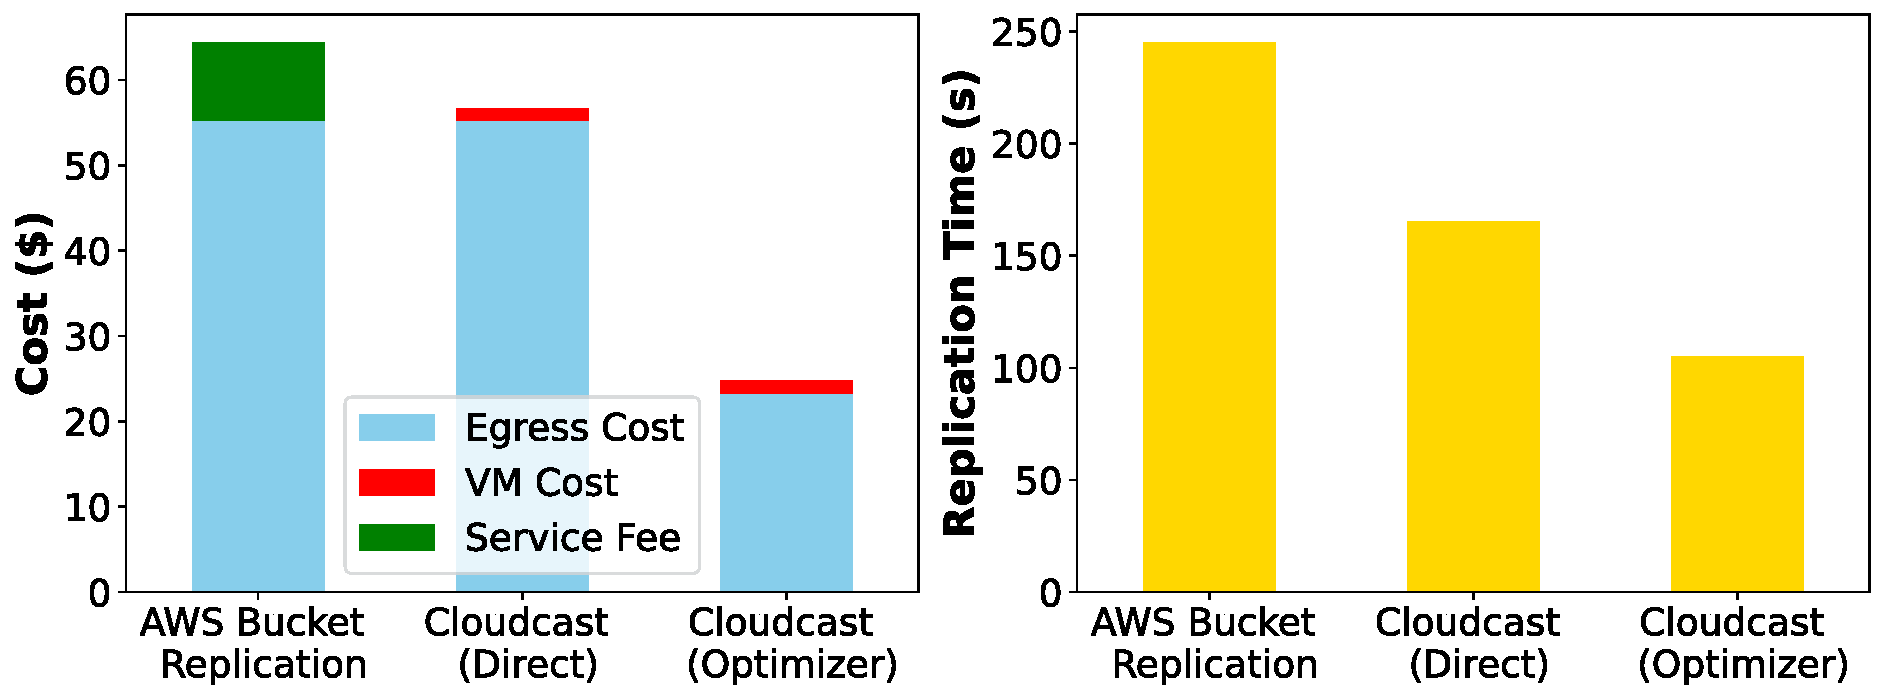
\includegraphics[width=
    \linewidth]{figures/opt_e2e.pdf}
    \caption{\textbf{Comparison with commercial baselines (6 VM per region limit):} We compare AWS bucket replication, \sys{} with a direct transfer tree and \sys{} with the optimizer. \sarah{consider adding skyplane baseline, or AWS DataSync? should mention how more vms = more speed}} 
    \label{fig:aws_comparison}
\end{figure}

\subsubsection{P2P Baseline: Bittorrent and Bullet}

We also compare \sys{} against P2P systems, BitTorrent and Bullet. 
%P2P systems are natural choices for transferring large files over multiple destinations. 
We run the same transfer benchmark in Azure in Figure \ref{fig:azure-intra-cloud}, sending 100GB within Azure to 6 destination regions. We host our own BitTorrent tracker and use aria2 (\cite{aria2}) as a BitTorrent client. Since Bullet's implementation is not available, we evaluate Bullet by implementing Bullet's algorithm inside \sys{}'s planner. The result is shown in \cref{fig:p2p_comparison}: both BitTorrent and Bullet have lower egress costs than direct but higher than \sys{}. BitTorrent is the slowest because most clients cannot utilize the full bandwidth. The clients are built for scenarios like background seeding and transfer off the critical path, rather than for bulk data transfer. Interestingly, without a centralized planner, BitTorrent is able to find a low-cost multicast replication tree by inferring the bandwidth among peers and preferring the data from peers who have the highest throughput. However, it is still significantly more expensive than \sys{}. 
%Peers also communicate with each other by requesting "pieces" and sending "choke" signals. The end result is an all-to-all communication graph that preferred high bandwidth regions like US, Canada, and Europe. 

\begin{figure}[t]
    \centering
    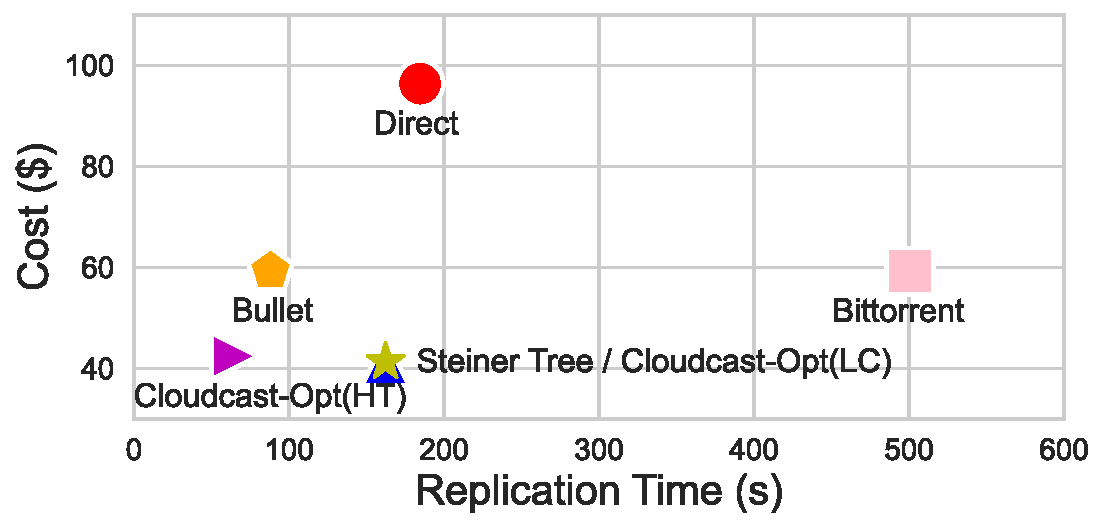
\includegraphics[width=0.75\linewidth]{figures/p2p-comparison-all.pdf}
    \caption{Comparison with BitTorrent protocol on the same transfer workload on Azure (\cref{fig:azure-intra-cloud}). 
    %BitTorrent is cost-conserving as compared to direct transfer. It has the highest runtime because the BitTorrent clients are not designed to efficiently utilize the full available bandwidth.
    }
    \label{fig:p2p_comparison}
\end{figure}

\subsection{Optimizer Performance}
In this section, we evaluate how our designed approximation techniques impact the optimizer solve time and solution quality, as well as how well the optimizer models throughput compared to the performance we observe in \sys{}. 
\subsubsection{How Do Approximations Affect Solver Runtime and Quality?} 
\label{sec:solution_qual_eval}
%As we described in \cref{ss:approximations}, the MILP formulation alone is not practical as a planning algorithm for \sys{} due to solver times that can take hours even for a few destinations. 

In this section, we evaluate how our approximations (node filtering via clustering, hop constraining, and stripe iterative) affect both the solution quality and solver runtime. 

We evaluate how the optimizer with and without approximations scales to larger numbers of destinations in Figure \ref{fig:solve_time}, by randomly selecting source and destination regions for varying numbers of destination regions. We can see from \cref{fig:solve_time} that combining all three approximation mechanisms is necessary to scale the optimizer. 

%For a given number of destinations, we sample a single random combination of source and destination regions, and measure the solver runtime with and without approximations, show in \cref{fig:solve_time}. We terminate the solver at 30 minutes if it cannot solve within that time. We find that we have to terminate the solver with no approximations with only 3 destinations. The stripe-iterative and node-clustering based approximations also can only run up to 7 and 14 destinations respectively and take 100s of seconds for higher numbers of destinations. However, if we combine all approximations together, we can solve for up to 20 destinations in a few seconds. 

\begin{figure}[t]
    \centering
    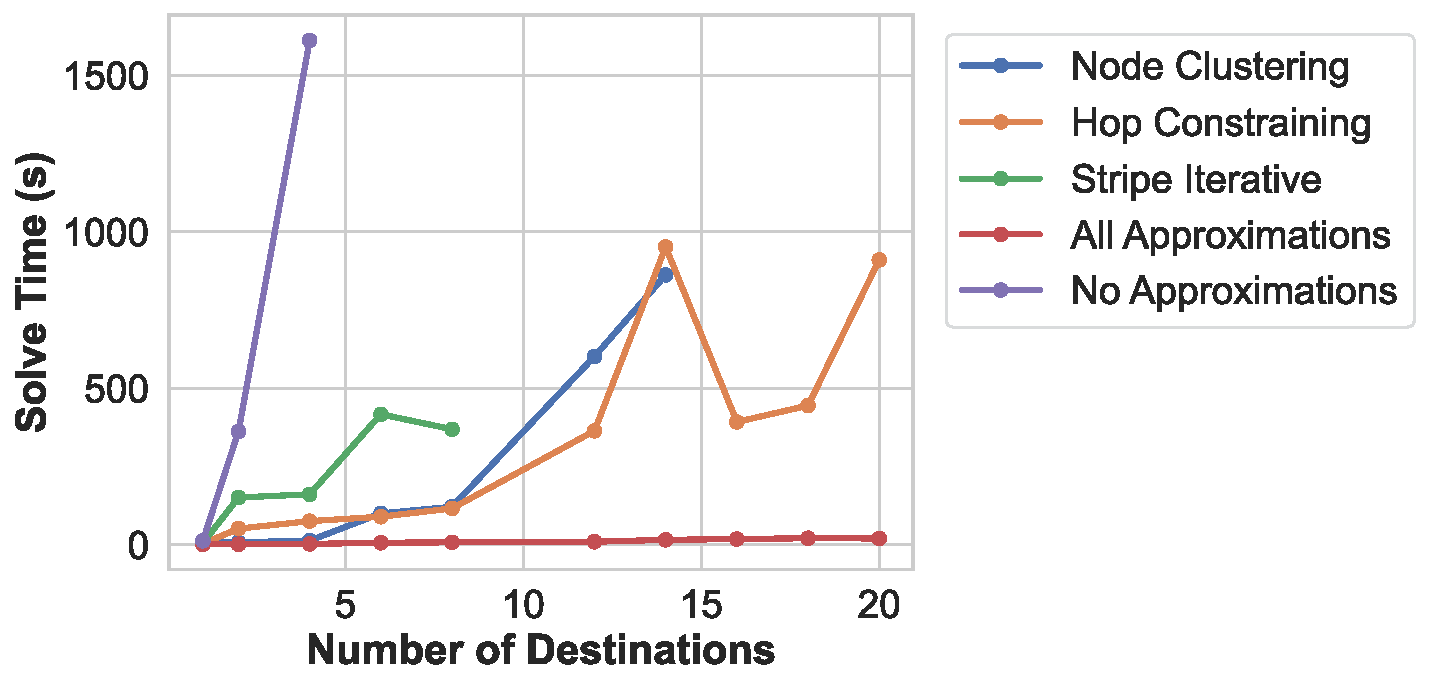
\includegraphics[width=\linewidth]{figures/solve_time_versus_num_dest.pdf}
    \caption{Solve Time v.s Number of Destinations: We run the solver with different approximation mechanisms and cutoff measurement at 30 minutes. Without approximations (in purple), the solve time quickly becomes untenable and cannot reach beyond 4 destinations. With approximations (in red), solve time is within a few seconds even for up to 20 destinations. }
    \label{fig:solve_time}
\end{figure}

We also evaluate how approximations affect the quality of the solution, but examining the cost of the solver-generated solution. We randomly sample 100 source/destination combinations for 5 destinations and compute the difference in solver cost and runtime compared to MILP without approximation in \cref{table:approx-quality}. We find that the difference in cost averages around $1\%$, and estimate the worst-case approximation ratio to be $1.4$. We find that for even just 5 destinations, the approximated solver runs with a geometric-mean speedup of $30.68\times$. As such, our approximations are reliable and fast.


% \begin{table}[]
% \label{table2}
% \resizebox{\linewidth}{!}{%
% \begin{tabular}{|l|lll|lll|}
% \hline
% \multirow{2}{*}{Approximation} & \multicolumn{3}{l|}{Relative Solve Quality (\%)}               & \multicolumn{3}{l|}{Relative Solve Time Speedup (\times)}        \\ \cline{2-7} 
%                             & \multicolumn{1}{l|}{Min} & \multicolumn{1}{l|}{Max} & Avg & \multicolumn{1}{l|}{Min} & \multicolumn{1}{l|}{Max} & Avg \\ \hline
% \textit{Node Clustering}                        & \multicolumn{1}{l|}{-1.2}    & \multicolumn{1}{l|}{22.7}    &   1.00  & \multicolumn{1}{l|}{-2.5}    & \multicolumn{1}{l|}{50.7}    &   9.04 \\ \hline
% \textit{Hop Constraining}                        & \multicolumn{1}{l|}{-1.2}    & \multicolumn{1}{l|}{44.5}    &   1.01  & \multicolumn{1}{l|}{-0.72}    & \multicolumn{1}{l|}{26.2}    &   5.72 \\ \hline
% \textit{Stripe Iterative}                         & \multicolumn{1}{l|}{-0.4}    & \multicolumn{1}{l|}{0.8}    &   0.02  & \multicolumn{1}{l|}{-0.78}    & \multicolumn{1}{l|}{47.5}    &  7.02 \\ \hline
% \textit{All Approximations}                  & \multicolumn{1}{l|}{-1.7}    & \multicolumn{1}{l|}{\textbf{44.4}}    &  \textbf{1.08}  & \multicolumn{1}{l|}{-4.9}    & \multicolumn{1}{l|}{\textbf{219.1}}   &  \textbf{30.68}   \\ \hline
% \end{tabular}
% }
% \label{fig:approx-quality}
% \caption{Approximation Solve Time and Quality: Compare solution cost and solver runtime with respect to the original MILP for 100 randomly generated 5-destination configurations. Note that since the original MILP itself is an approximation, we are approximating an approximation, so the minimum is sometimes negative (i.e. it is not guaranteed the approximations result in worse solutions).}
% \end{table}
\begin{table}[]
\centering
\caption{An ablation of approximation methods demonstrates the substantial solve time reductions are possible without a significant decrease in solution quality.}
\label{table:approx-quality}
\begin{tabular}{lcc}
\toprule
\textbf{Method} &
  \multicolumn{1}{c}{\textbf{Error (mean)}} &
  \multicolumn{1}{c}{\begin{tabular}[c]{@{}c@{}}\textbf{Solver speedup}\\ \textbf{(geomean)}\end{tabular}} \\ \midrule
\textit{Node Clustering}    & 0.3\% & 9.04$\times$  \\
\textit{Hop Constraining}   & 1.1\% & 5.72$\times$  \\
\textit{Stripe Iterative}   & 0.0\% & 7.02$\times$  \\
\cellcolor{Gray} \textit{All Approximations} & \cellcolor{Gray} 1.1\% & \cellcolor{Gray} 30.68$\times$ \\ \bottomrule
\end{tabular}%
\end{table}

%A challenge with making the optimizer practical for real-world use cases is having sufficiently low runtime even for large numbers of destinations and stripes. We reduce the runtime using approximation mechanisms described in \ref{reduce_optimizer_runtime}. We show how approximation mechanisms affect solver quality (in terms of the cost of the solution) and solver runtime in \cref{fig:approx-quality}. 


\subsubsection{How well can our optimizer predict replication throughput?}
Modeling replication throughput is the key to ensuring that optimizer solutions meet replication time constraints.  We show a comparison between optimizer-modeled throughput and real throughput in \cref{table:tp-prediction}. As transfer size increases, the approximation becomes more accurate. This is because we design our optimizer in the context of bulk data replication, assuming that stripes are perfectly pipelined. As a result, for smaller transfers, throughput in \sys{} is less than what is modeled with the optimizer. However, for larger data transfers, the modeled expected throughput is able to match the real system throughput.
%fig:simulator_accuracy (old figure) 

% \textcolor{red}{Sarah: Why is there still overhead for larger transfer sizes?} 



\begin{table}[tbp]
\label{table:tp-prediction}  
\begin{center}  
\caption{The optimizer's predicted throughput is accurate for large bulk transfers but may not accurately model small files.}
\begin{tabular}{cc}  
  
\toprule % Toprule applied here  
  
Transfer Size (GB) & \begin{tabular}[c]{@{}c@{}}Error for predicted\\ throughput\end{tabular} \\  
  
\midrule % Midrule applied here  
   
 16 & 16.6\%\\  
 32 & 8.51\%\\  
 64 & 3.31\% \\  
 128 & 1.69\%\\  


\bottomrule % Bottomrule applied here  
\end{tabular}  
\end{center}  
\end{table} 

% \begin{figure}[t]
%     \centering
%     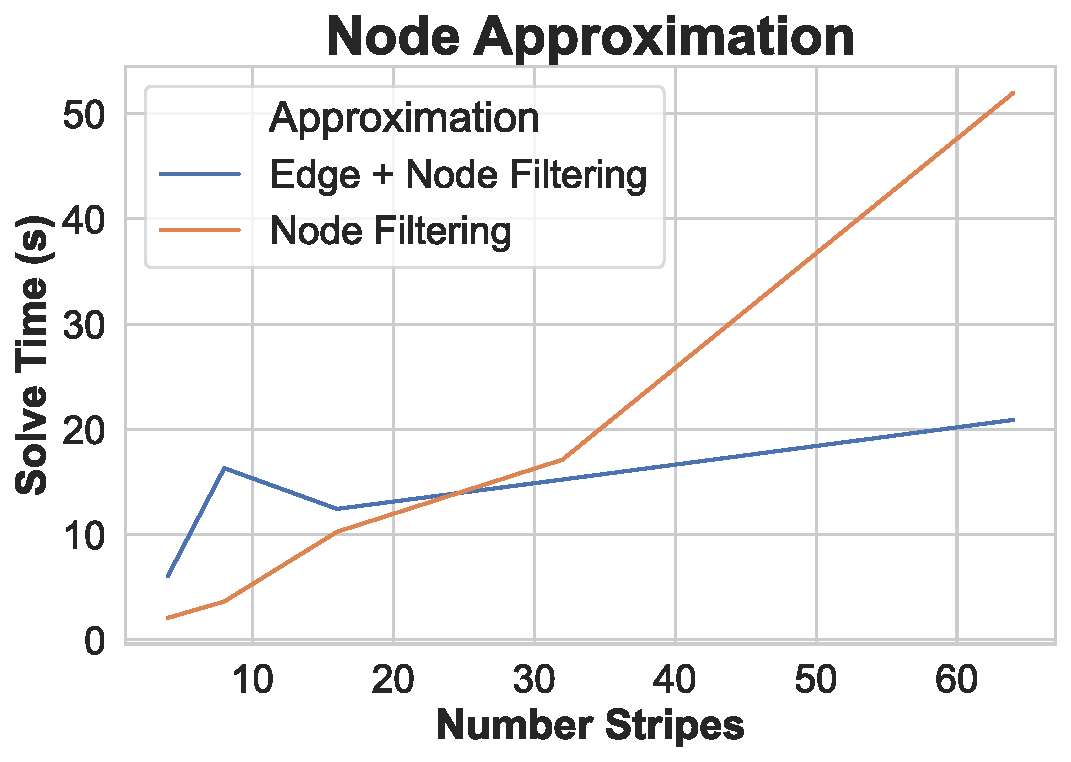
\includegraphics[width=.75\linewidth]{figures/node_approx.pdf}
%     \caption{\textbf{Quality of approximation techniques (showing 100 configs, 6-dest result)}}
%     \label{fig:node_approx}
% \end{figure}



